\begin{tikzpicture}
  \node[anchor=south west, inner sep=0] (image) at (0, 0) {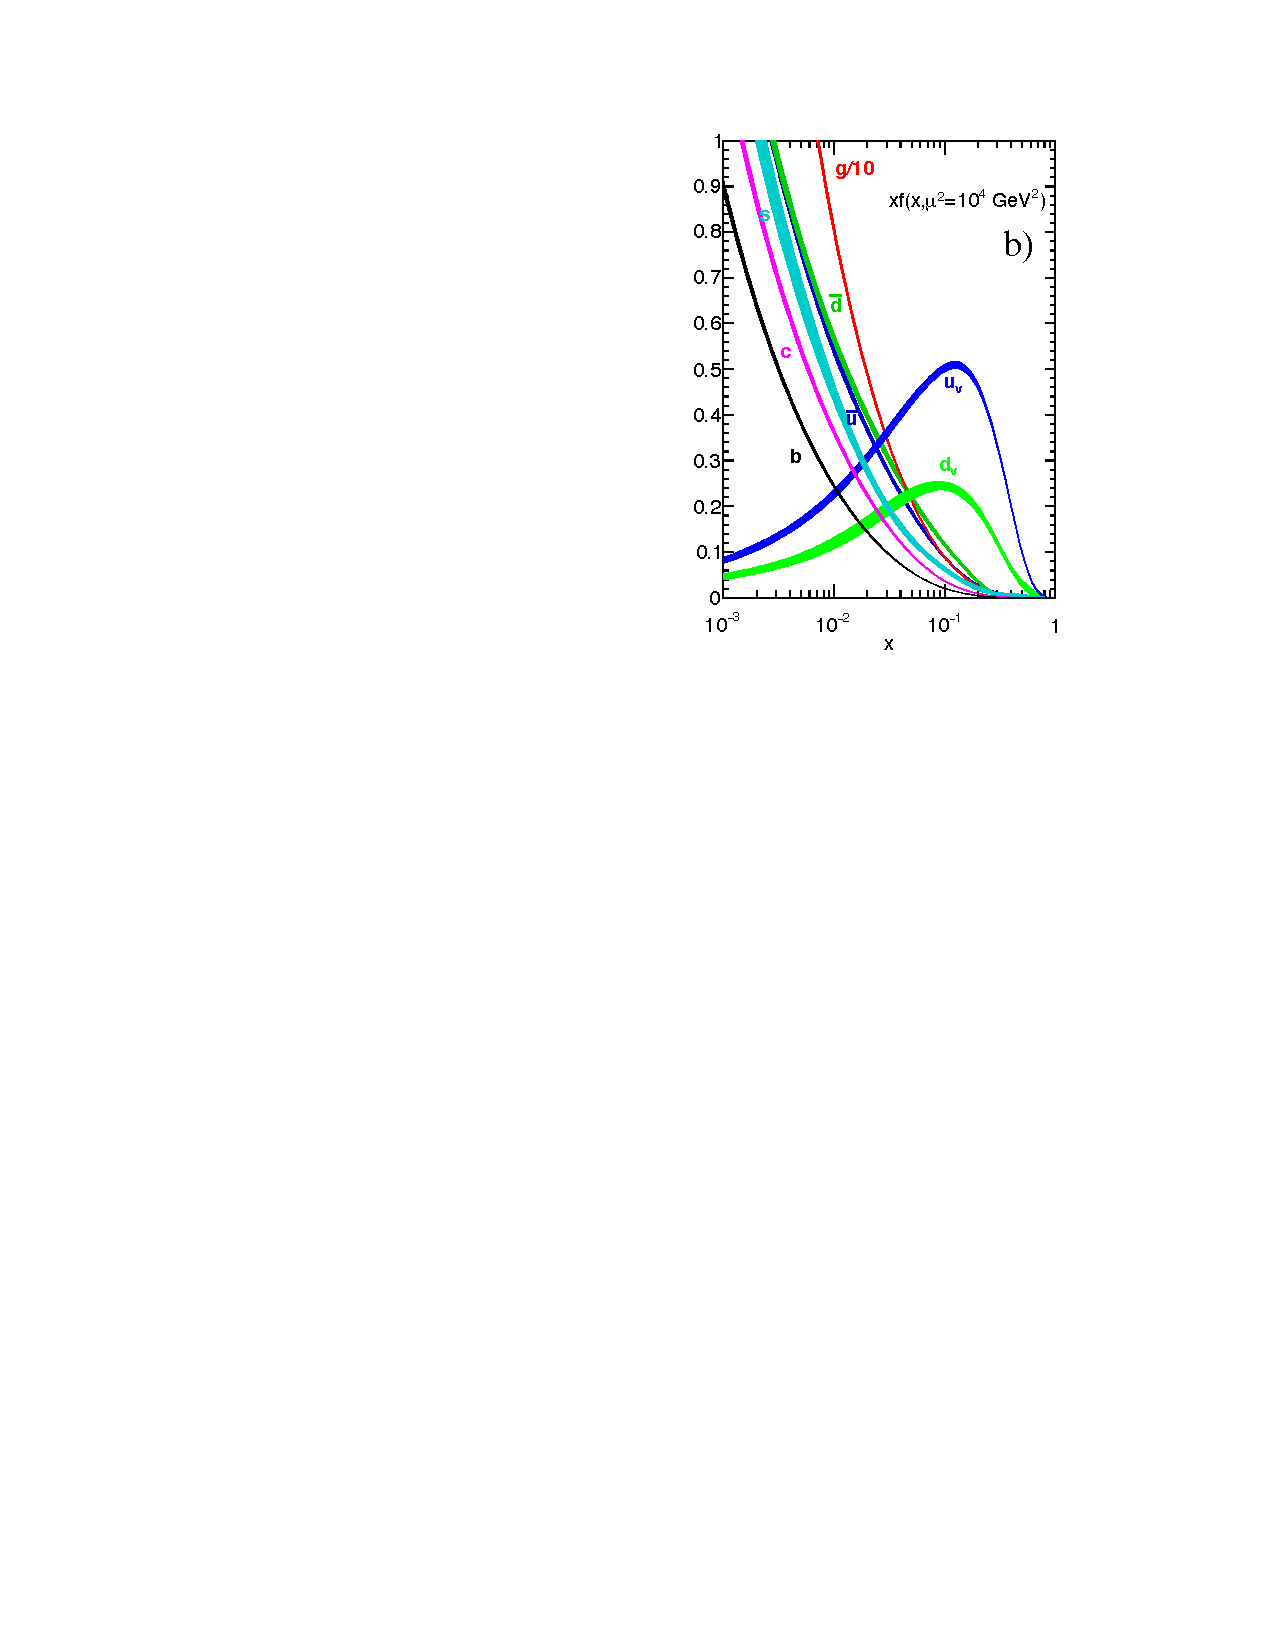
\includegraphics[width=0.9\textwidth]{production/pdf_sets_high_qsquared}};
  \begin{scope}[x={(image.south east)}, y={(image.north west)}]
    % Grid to help find coordinates on the image
    % \draw[step=0.02, gray, very thin] (0, 0) grid (1, 1);
    % Box to cover xf function label
    \path[fill=white] (0.52, 0.84) rectangle (0.96, 0.90);
    % Box to cover 'b)' label
    \path[fill=white] (0.82, 0.74) rectangle (0.94, 0.82);
    % Q^2 label
    \node[anchor=south west] at (0.54, 0.79) {\footnotesize\begin{sansmath}$Q^{2} = \SI{e4}{\GeV\squared}$\end{sansmath}}; 
    % y-axis label
    \node[rotate=90] at (-0.05, 0.5) {\footnotesize\begin{sansmath}$xf(x, Q^{2})$\end{sansmath}};
  \end{scope}
\end{tikzpicture}
